% !TeX spellcheck = de_CH
\documentclass[
a4paper,
oneside,
landscape, 
fontsize=8pt,
]{scrartcl}

% language
\usepackage[T1]{fontenc}
\usepackage[utf8]{inputenc}

% tables
\usepackage{tabu}
\usepackage{booktabs}
\tabulinesep=1.2mm

% images
\usepackage{graphicx}

% layout
\usepackage[landscape]{geometry}
\geometry{tmargin=5mm,bmargin=5mm,lmargin=5mm,rmargin=5mm}
\usepackage{multicol}
\setlength{\columnsep}{1cm}

% math
\usepackage{amsmath}
\usepackage{amssymb}
\usepackage{amsfonts}
\usepackage{enumitem}

% include pdf as-is
\usepackage{pdfpages}
 
% title
\title{PhAI: Physik Anwendungen für Informatiker}
\subject{Cheatsheet}
\author{Michael Wieland, Demian Thoma \& Lukas Röllin}
\date{\today}


\begin{document}

\maketitle


\begin{multicols*}{2}
	
\tableofcontents
\clearpage
	
\section{Grundlagen der GUI Programmierung}
Apps bestehen aus lose gekoppelten, wiederverwendbaren Komponenten. Diese sind Activities (für den Benutzer sichtbar) und Services, Content Provider, Broadcast Receivers (unsichtbar für Benutzer). Das System hat die Kontrolle über alle Applikationen und Verwaltet den Lebenszyklus, ist verantwortlich für die Kommunikation zwischen Komponenten und schliesst die Apps automatisch um Speicher zu sparen.
\paragraph{Activites} Dies sind die Hauptbausteine in der App Entwicklung, die Activity interagiert mit dem Benutzer. Eine Activity stellt immer auch einen möglichen Eintrittspunkt in die App ein.
\begin{lstlisting}[language=java]
public class MainActivity extends Activity {
  @Override
  protected void onCreate(Bundle savedInstanceState) {
    super.onCreate(savedInstanceState);
    /* ... */
  }
}
\end{lstlisting}
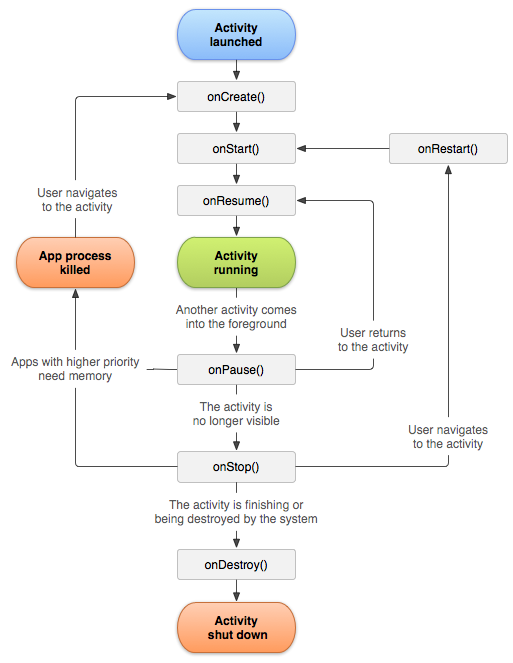
\includegraphics[scale=0.35]{activity_lifecycle.png}
Unterschied Paused/Resume: wird die Activity von einer anderen überdeckt (z.B. Notificationleiste heruntergezogen), wird die erste pausiert (\code{onPause}). Kommt sie wieder in den Vordergrund, wird wieder \code{onResume} aufgerufen.

\code{onPause} ist \textbf{garantiert}. \code{onStop} ist jedoch \textbf{nicht garantiert}. Darum:

\paragraph{Best Practice}

\begin{itemize}
  \item \code{onCreate} erstellt GUI beim Start.
  \item \code{onResume} reagiert auf Benutzereingaben.
  \item \code{onPause} sichert Daten (da die App auch im \code{onStop} oder \code{onDestroy} gekillt werden kann).
  \item \code{onStop} gibt Ressourcen frei.
\end{itemize}

Bei Konfigurationsänderungen wird die Activity neu gestartet. Dazu zählen z.B. \textbf{Screenausrichtungsänderungen}.

Stopped/Started: kommt die Activity wieder in den Vordergrund, weil der User die Applikation nochmal startet oder mit dem Back-Button zurückkommt, wird onRestart aufgerufen.

Destroyed: die App wird vom System destroyed, oder wenn sie explizit vom User geschlossen wird.

\paragraph{Stack}

Activities werden in einem Stack verwaltet, wobei die Activites eines Stacks zu verschiedenen Apps gehören können.\\ 
Eine Gruppe von Activities in einem Stack nennt man auch \textbf{Task}. Es können mehrere Tasks gleichzeitig existieren. Tasks lassen sich im Overview Screen anzeigen.

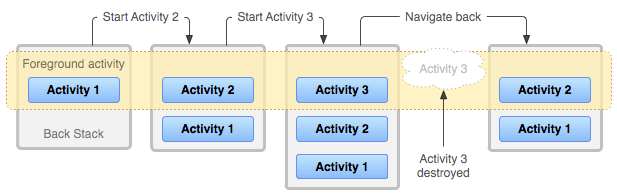
\includegraphics[scale=0.29]{diagram_backstack.png}

\paragraph{Activity Launch Modes} Activities haben verschiedene Launch Modes

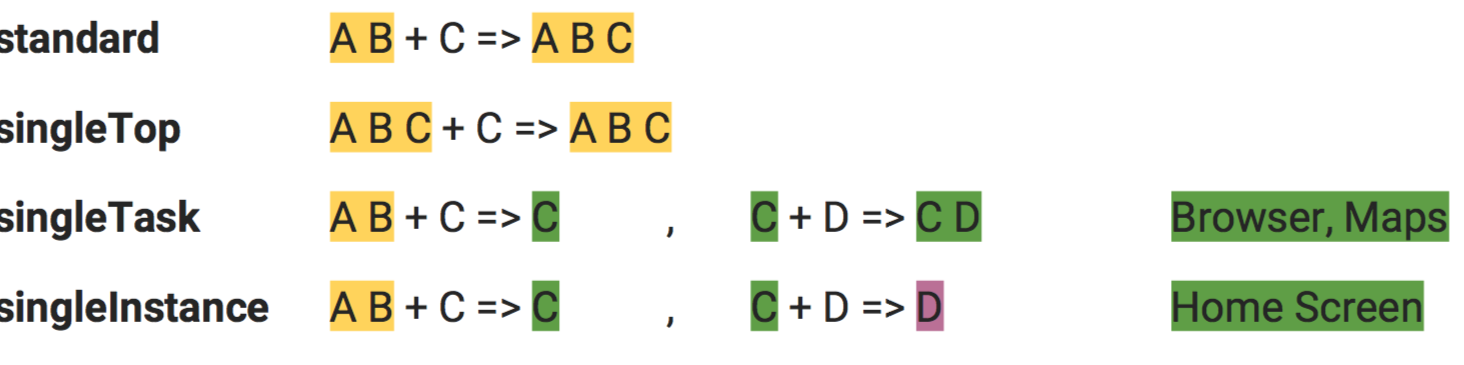
\includegraphics[scale=0.11]{activity-launch-modes.png}

\begin{itemize}
\item \textbf{Standard:} Es wird eine neue Activity in den Stack gepusht
\item \textbf{SingleTop:} Ist Activity A zuoberst auf dem Stack und sie wird nochmals gestartet, wird in Activity A \code{onNewIntent()} ausgeführt
\item \textbf{SingleTask:} Das System erstellt einen neuen Task und instanziert die Activity als die Root des neuen Tasks. Wenn aber schon eine Instanz dieser Activity existiert, wird \code{onNewIntent()} in dieser aufgerufen. 
\item \textbf{SingleInstance:} Es darf nur eine Instanz der Activity geben
\end{itemize}

\paragraph{APK}

Activities (und Ressourcen, etc) werden in ein APK gepackt und installiert. Wird eine Activity aktiv, wird pro APK ein Linux Prozess mit einem Thread gestartet, welcher alle Activities die indiesem APK enthalten sind ausführt. Jedes APK wird unter einem eigenen Linux-User installiert. Inhalt: Libraries, Ressourcen, Assets, Metadaten, kompilierte Klassen im DEX-Format.

Ein APK ist nichts anderes als ein JAR, welches wiederum eine ZIP-Datei ist.

\subsection{Application}
Parent unserer Activities im Manifest ist die Application. Ist auch eine Klasse, die den globalen Zustand unserer App hält. Kann durch eigene Application-Subklasser ersetzt werden. Zugriff aus Activity mit \code{getApplication}, Lifecycle-Methoden: \code{onCreate}, \code{onLowMemory}, \code{onConfigurationChanged}.


\paragraph{Intent} Ein Intent beschreibt was gemacht werden soll und das System entscheidet wer zuständig ist. Apps können selbst wiederum Activites zur Verfügung stellen und bestehende Applikationen ersetzen. Andere Activities können explizit oder implizit aufgerufen werden:
\begin{lstlisting}[language=java]
// Explizit mit Klasse
Intent in = new Intent(this, CalculateActivity.class)
// Implizit mit Aktion
Intent in = new Intent(MediaStore.ACTION_IMAGE_CAPUTRE)
\end{lstlisting}
Andere Activities kann man mit \code{startActivity(intent)} oder \code{startActivityForResult(intent, myId)} starten. Um bei letzterem mit dem Rückgabewert arbeiten zu können muss man \code{onActivityResult} überschreiben.
\begin{lstlisting}[language=java]
@Override
protected void onActivityResult(int request, int result, Intent data) {
  if (result == Activity.RESULT_OK && request == myId) {
    /* ... */
  }
}
\end{lstlisting}
Möchte man einem Intent Daten übergeben, kann man das entweder mit der \code{setData} Methode, welche eine URI entgegennimmt, oder mit \code{putExtra(MediaStore.EXTRA\_OUTPUT, imageCaptureUri)}. Letzere ist eine Struktur mit Key-Value Paaren und nimmt nur primitive Daten, Strings und serialisierbare Datentypen an.

\paragraph{Manifest} Das Manifest enthält Meta-Daten einer App. Es umfasst
\begin{itemize}
\item Komponenten der App
\item Metadaten (Name, Icon, Versionsnummer)
\item Permissions (Internet, kostenpflichtige Anrufe etc.)
\item Anforderungen an die Geräte API
\item \code{minSdkVersion} min-Version des Gerätes
\item \code{targetSdkVersion} höchste Version, mit der getestet wurde
\item Name der Singleton Instanz der Application (Sub-)Klasse.
\end{itemize}

Das Manifest wird vom System verwendet um zu wissen, ob die App installiert werden kann, welche Permissions diese verwendet etc.

\subsection{Android GUI}
\paragraph{Aufbau} Die Basisklasse um User Interfaces zu bauen ist die \code{View}. Eine View ist zuständig seinen Inhalt zu zeichnen und Events zu behandeln. Untergruppen der View sind Widgets und ViewGroups. Widgets ist ein Sammelbegriff für alle fix-fertigen Komponenten für User-Interfaces (Buttons, Images, Checkboxes etc.)
\paragraph{ViewGroup} Die ViewGroup ist eine Unterklasse von View. Sie kann andere View beinhalten. Wenn die ViewGroup beinhaltende View anordnet, spricht man von einem Layout.
\paragraph{Basis Layout} Layouts sind ViewGroups und beschreiben die visuelle Struktur des UIs.
\includegraphics[scale=0.45]{layouts.png}
Die Layout-Parameter beschreiben wie die Views angeordnet und dargestellt werden. Für alle ViewGroups gemeinsam sind \code{android:layout\_width} und \code{android:layout\_height}. Häufig benutze Werte sind \code{match\_parent} (So gross wie mögich, also wie der Parent erlaubt) und \code{wrap\_content} (so klein wie möglich, also wie die Kinder erlauben).\\
In einem \textbf{Linear Layout} werden die Elemente horizontal oder vertikal angeordnet. Mit \code{android:layout\_weight} kann man Elementen ein Gewicht geben, da es selten sinnvoll ist, alle Elemente gleich gross zu lassen. Kinder ohne Weight bekommen minimalen Platz, auf die restlichen wird der verfügbare Platz nach Gewicht aufgeteilt.\\
Das \textbf{Relative Layout} ist das vielseitigse Layout welches Kinder relative zueinander anordnet.
\begin{lstlisting}[language=xml]
<RelativeLayout xmlns:android="... >
  <TextView
    android:text="1. Platz"
    android:id=@+id/first"
    android:layout_centerHorizontal="true" />
  <TextView
    android:text="2. Platz"
    android:id="@+id/first"
    android:layout_below="@id/first"
    android:layout_toStartOf="@id/first" />
  <TextView
    android:text="3. Platz"
    android:id="@+id/textView3"
    android:layout_below="@id/first"
    android:layout_toEnfOf="@id/first" />
</RelativeLayout>
\end{lstlisting}
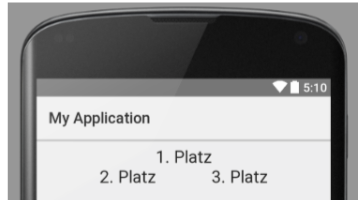
\includegraphics[scale=0.25]{RelativLayout.png} \\
Das \textbf{Frame Layout} kann die Kinder übereinander anordnen (Hilfslinien bei einer Kamera-App).\\
Das Layout muss in der Activity deklariert werden. Dies wird in der Activit Klasse mit \code{setContentView(R.layout.activity\_main)} gemacht.\\

\paragraph{Weitere Layouts}
\begin{itemize}
  \item FlexboxLayout: CSS Flexbox
  \item ConstraintLayout, mit RelativeLayout verwandt (war in Android Studio immer Standard ab irgendeiner Version)
  \item WebView um HTML anzuzeigen: JavaScript kann aktiviert werden, und Java-Objekte können mit JS angesprochen werden
\end{itemize}

\subsection{View finden}
\begin{lstlisting}[language=java]
Button button = (Button) findViewById(R.id.button)
\end{lstlisting}
findViewById innerhalb einer Activity sucht im aktuellen Layout (wahrscheinlich dasjenige von \code{setContentView}). Rückgabe ist immer die Oberklasse \code{View},  das Resultat muss also noch gecastet werden.

Hat man allerdings ein Fragment oder z.B. ein Listenelement, so muss man die Parent-View vorher gespeichert haben (z.B. die Rückgabe des \code{LayoutInflater}), und dann auf dieser die gewünschte View finden. 

\subsection{Widgets}
\paragraph{Button} Vom Button gibt es einen normalen \code{Button} und einen \code{ImageButton} bei dem man mit dem \code{android:src} ein Bild einfügen kann.
\paragraph{Eingabefelder} Der Typ des Eingabefeld bestimmt welche Tastatur verwendet wird. Dies kann man mit dem \code{android:inputType} bestimmen, z.B. \code{textCapSentences}. Es sind auch Kombinationen möglich, z.B. \code{textCapSentences | textAutoCorrect}
\paragraph{Referenzen und ID} Möchte man GUI-Elemente referenzieren, gibt man ihnen einen ID-String, welche Strings sind, die mit \code{@} beginnen. Wenn man einen neue ID definieren will, macht man das mit \code{@+id/}. Das Android-Buildsystem sammelt alle diese IDs als Konstanten in der automatisch generierten Klasse R. Diese Klasse enthält alle Ressourcen als Konstanten. Weitere Resourcesn sind: \code{drawable} (Bilder), \code{menu} (Menüs), \code{mipmap} (Launcher Icon der App) und \code{values} (Strings und andere Konstanten). Mit Aussnahme der values, wird für jeden Ordner eine innere Klasse in R generiert.
\paragraph{Dimensionen in Ressourcen} Konstanten in \code{dimens.xml} werden für Grössen in den Layouts benutzt.
Die Ordnernamen müssen in Java-Namen umgewandelt werden können, dürfen also z.B. kein \code{-} enthalten.

Ressourcen können in mehreren Varianten vorliegen. Die Ordnernamen unterliegen Konventionen, mit denen z.B. Ressourcen-XML für Tablets erstellt werden können, die dann andere Grössenangaben haben.

\begin{lstlisting}[language=xml]
<!-- Layout -->
<RelativeLayout xmlns:android="..." xmlns:tools="..."
  android:layout_width="match_parent"
  android:layout_height="match_parent"
  android:paddingLeft="@dimen/activity_horizontal_margin"
  android:paddingRight="@dimen/activity_horizontal_margin"
  android:paddingTop="@dimen/activity_vertical_margin"
  android:paddingBottom="@dimen/activity_vertical_margin"
  tools:context=".MainActivity">
<!-- dimens.xml -->
  <!-- Default screen margins, per the Android Design guidelines. -->
  <dimen name="activity_horizontal_margin">16dp</dimen>
  <dimen name="activity_vertical_margin">16dp</dimen>
</resources>
\end{lstlisting}
Grössenangeben von Views erfolgen in density-indepentent Pixels (dp oder dip). Bei Schriften verwendet man scale-independent Pixels (sp).
\paragraph{Events und Event Handling}\label{grundlagen:eventhandling} Das Android-Framework hat einen sogenannten Event-Loop (Looper). Dieser wartet bis ein Ereignis passiert und verarbeitet dieses dann. Nur der Main-Thread darf das GUI verändern. \\
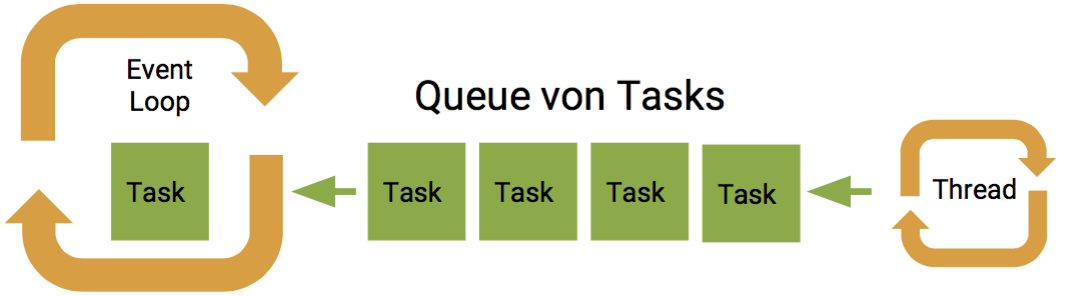
\includegraphics[scale=0.25]{EventLoops.png} \\
Fast alle Listener können mit \code{set[EventName]Listener} registriert werden.
\begin{lstlisting}[language=java]
button.setOnClickListener(new View.OnClickListener() {
  @Override
  public void onClick(View v) {
    /* ... */
  }
});
\end{lstlisting}
Oder onClick Listener in XML deklariert
\begin{lstlisting}[language=xml]
android:onClick="onButtonClicked"
\end{lstlisting}
Alternativ zur anonymen Klasse, kann die Activity auch das Interface implementieren, das kann man mit  (\code{setOnClickListener(this))} bekannt machen.

Ein Listener lässt sich auch bei mehreren Views registrieren. Mit dem übergebenen \code{View}-Parameter kann man unterscheiden (Referenz-Vergleich \code{==}) welches Element den Event ausgelöst hat.

\paragraph{TextWatcher}
Bei der Verarbeitung von Texteingaben haben wir mehrere Möglichkeiten auf Events zu reagieren. Das zu implementierene Interface (\code{TextWatcher}) umfasst 3 Methoden:
\begin{itemize}
\item \code{beforeTextChanged}: Wird aufgerufen bevor der Text geändert wird
\item \code{onTextChanged}: Wird aufgerufen sobald der Text geändert hat
\item \code{afterTextChanged}: Nachdem der Text geändert wurde, kann man den Text noch anpassen (Loop-Gefahr)
\end{itemize}
\begin{lstlisting}[language=java]
editText.addTextChangedListener(new TextWatcher() {
  public void onTextChanged(CharSequence s, int start, int before, int count){ }
  public void beforeTextChanged(CharSequence s, int start, int count, int after){ }
  public void afterTextChanged(Editable s) { }
});
\end{lstlisting}
Bei Eingabefeldern kann man mit \code{setError} Meldungen anzeigen lassen. Dies eignet sich gut für eine Inputvalidierung. Bei jeder Änderung wird diese zurückgesetzt.
\begin{lstlisting}[language=java]
final EditText password = (EditText) findViewById(R.id.password);
password.addTextChangedListener(new TextWatcher() {
  @Override
  public void afterTextChanged(Editable s) {
    String pw = s.toString();
    if (s.length() < 8) {
    password.setError("Passwort muss mindestens 8 Zeichen lang sein.");
    }
  }
  ...
});
\end{lstlisting}
\subsection{Android Testing mit JUnit}
Es gibt mehrere Arten von Tests für eine Activity. Die \code{ActivityUnitTest} manipulieren das UI im Code, die \code{ActivityInstrumentationTestCase2} schickt Clicks und Events an das UI. Um eine App mit mehreren Activities zu testen, gibt es das Espresso Framework, sowie UI Automator um App-übergreifend zu testen.
\begin{lstlisting}[language=java]
public class MainActivityLayoutTest extends ActivityUnitTestCase<MainActivity> {
  public MainActivityLayoutTest() {
    super(MainActivity.class);
  }
  @Override
  protected void setUp() throws Exception {
    super.setUp();
    ContextThemeWrapper context = new
      ContextThemeWrapper(getInstrumentation().getTargetContext(), R.style.AppTheme);
    setActivityContext(context);
    startActivity(
      new Intent(getInstrumentation().getTargetContext(), MainActivity.class),null,null);
}
\end{lstlisting}
Funktionale Tests (ActivityInstrumentationTestCase2) testen eine Activity im echten Systemkontext. Der Test löst Events aus und prüft, ob diese zum erwünschten Resultat führen. Dazu gehören: 
\begin{itemize}
\item Ändert sich das UI wie erwartet
\item Überprüfen von Inputvalidierung
\item Werden Lifecycle Events korrekt behandelt
\end{itemize}
\begin{lstlisting}[language=java]
public class MainActivityInteractionTest extends ActivityInstrumentationTestCase2<MainActivity> {
  public MainActivityInteractionTest() { super(MainActivity.class); }
  public void testSayHi() {
    MainActivity activity = getActivity();
    final EditText editText = (EditText) activity.findViewById(R.id.editText);
    getInstrumentation().runOnMainSync(new Runnable() {
      @Override
      public void run() {
        editText.requestFocus();
      }
    });
    getInstrumentation().waitForIdleSync();
    getInstrumentation().sendStringSync("Hello");
    getInstrumentation().waitForIdleSync();
    Button button = (Button) activity.findViewById(R.id.button);
    TouchUtils.clickView(this, button);
...
\end{lstlisting}


\clearpage

\section{Mechanik}

\subsection{Statik}

\subsubsection{Drehmoment}

\begin{itemize}
	\item Die wirksame Hebellänge wird begrenzt zwischen dem Drehpunkt und dem Ansatzpunkt der Kraft
	\item Mehrere Drehmomente im Gegenuhrzeigersinn (positives Vorzeichen) und im Uhrzeigersinn (Vorzeichen) sind im Gleichgewicht, wenn das Gesamtdrehmoment $M_{tot}$ null ist.
	\item \textbf{Hebelgesetz}: Kraft $\cdot$ Kraftarm = Last $\cdot$ Lastarm
	\item Der Bezugspunkt P ist frei wählbar
	\item Das Drehmoment ($M = J \alpha$) ist für die Rotation, die Kraft in der Translation ($F = ma$)
\end{itemize}

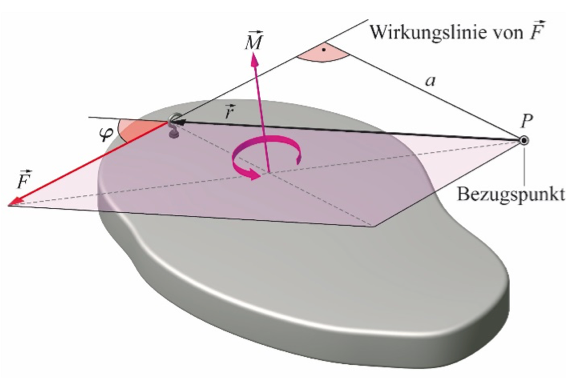
\includegraphics[width=0.4\linewidth]{images/drehmoment}

\begin{tabbing}
	\begin{tabu} to \linewidth {l X l X}
		\toprule
		Hebelgesetz & $F_1l_1 = F_2l_2 \Leftrightarrow M_1 = M_2$ & 
		Drehmoment & $M = F \cdot r \cdot \sin(\varphi)$ \\
		Drehmoment & $M = J \cdot \alpha$ & 
		Trägheitsmoment & $J = m r^2$ \\
	\end{tabu}
\end{tabbing}

\begin{tabbing}
	\begin{tabu} to \linewidth {l X l}
		Variable & Bedeutung & SI-Einheit \\
		\midrule
		$M$ & Drehmoment & $Nm$ \\ 
		$F$ & wirkende Kraft & $Nm$ \\ 
		$r$ & Abstand Bezugspunkt-Angriffspunkt & $m$ \\ 
		$a$ & Hebelarm: senkrechter Abstand Bezugspunkt-Wirkungslinie der Kraft & $m$ \\ 
		$P$ & Bezugspunkt: Frei wählbar & \\
		\bottomrule
	\end{tabu}
\end{tabbing}


\begin{minipage}[h!]{0.5\linewidth}
	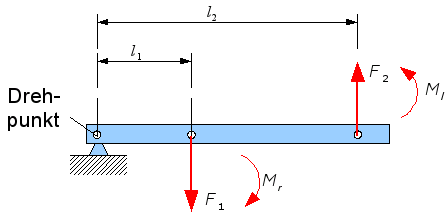
\includegraphics[width=0.8\linewidth]{images/hebel_einseitig}
\end{minipage}
\hfill
\begin{minipage}[h!]{0.5\linewidth}
	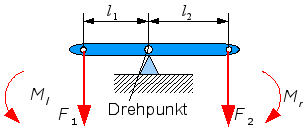
\includegraphics[width=0.8\linewidth]{images/hebel_zweiseitig}
\end{minipage}



\begin{minipage}[h!]{0.5\linewidth}
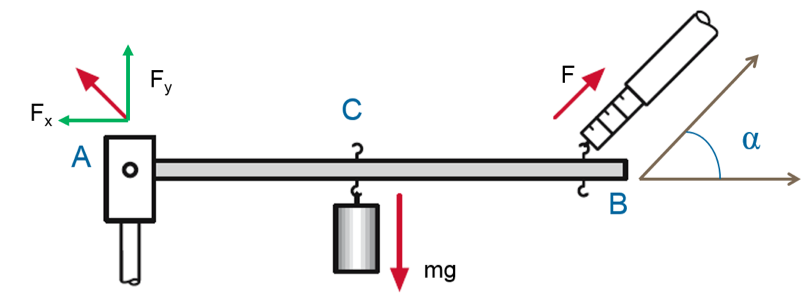
\includegraphics[width=0.9\linewidth]{images/hebel}
\end{minipage}
\hfill
\begin{minipage}[h!]{0.5\linewidth}
	
	\begin{align*}
	M_A &:	F  \cdot r \cdot  \sin(\alpha) - m g \cdot \frac{r}{2} = 0 \\
	\Rightarrow F &= \frac{mg}{2 \sin(\alpha)} \\
	X&:	F \cos(\alpha) - F_x = 0 \\ 
	Y&:	F \sin(\alpha) + F_y - m g = 0 \\ 
	\Rightarrow F_x &= F \cos(\alpha) \text{ und } F_y = mg - F \sin(\alpha) \\
	\Rightarrow F_{t} &= F_1 + F_2 \\
	\end{align*}
	
\end{minipage}

\subsubsection{Gleichgewicht}

Ein Massenpunkt ist im Gleichgewicht wenn die Summe der Kräfte gleich null ist. 

\begin{tabbing}
	\begin{tabu} to \linewidth {l X}
		\toprule
		Kräftegleichgewicht & 
		$\vec{F}_{res} = \vec{F}_1 +\vec{F}_2 + .. + \vec{F}_n \Rightarrow  \sum_{i=1}^{n}\vec{F}_i = \vec{0}
		\Rightarrow  \sum_{i=1}^{n}\vec{M}_i = \vec{0}$ \\
		Massenmittelpunkt & $\sum_{i=1}^{n} \frac{r_i \cdot m_i}{m_ges}$ \\
		\bottomrule
	\end{tabu}
\end{tabbing}

\begin{tabbing}
	\begin{tabu} to \linewidth {l X l}
		Variable & Bedeutung & SI-Einheit \\
		\midrule
		$m_i$ & Massenelemente &  \\ 
		$r_i$ & Ortsvektoren der Massenelemente &  \\ 
		\bottomrule
	\end{tabu}
\end{tabbing}

Die Summe muss mit Vektoraddition ausgerechnet werden. Nach Festlegung eines Koordinatensystems kann mit Komponenten der Vektoren gerechnet werden. In zwei Dimensionen erhalten wir somit zwei Gleichungen und können maximal zwei Unbekannte bestimmen.


\begin{minipage}[h!]{0.5\linewidth}
	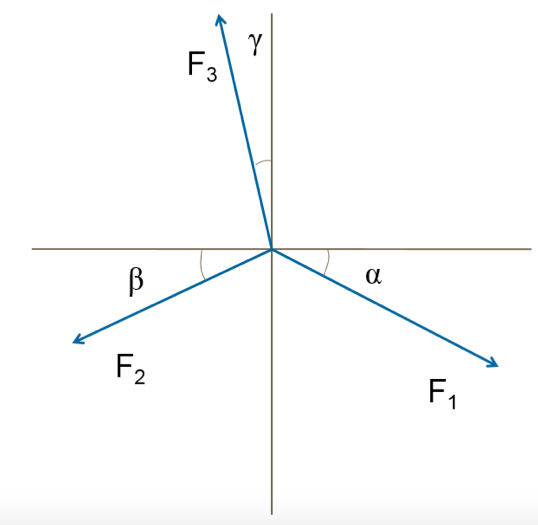
\includegraphics[width=0.7\linewidth]{images/gleichgewicht}
\end{minipage}
\hfill
\begin{minipage}[h!]{0.5\linewidth}
	
	\begin{align*}
	X &: F_1  \cos(\alpha) - F_2  cos(\beta) - F_3 \sin(\gamma) = 0 \\
	Y &: -F_1  \sin(\alpha) - F_2 \sin(\beta) + F_3 \cos(\gamma) = 0
	\end{align*}
	
\end{minipage}

\subsubsection{Schwerpunkt}
Die Gewichtskraft eines Körpers ist gleich der Summe der Gewichtskräfte seiner Teilchen. Die Summe der Gewichtskräfte greift im Schwerpunkt an.

\begin{itemize}
	\item Wenn ein Körper im Schwerpunkt aufgehängt wird, ist er im Gleichgewicht. Somit ist das Drehmoment um den Schwerpunkt = 0
	\item Die Schwerkraft, welche auf einen starren Körper wirkt, kann durch eine Kraft im Schwerpunkt ersetzt werden. $r_p \sum_{i} m_i = \sum_{i} m_i  r_i$
\end{itemize}



\clearpage


\subsection{Kinematik}
Man unterscheidet zwei Arten von Bewegungen:
\begin{itemize}
	\item Translation (geradlinige Bewegung)
	\item Rotation (Drehbewegung)
\end{itemize}

Die meisten Kinematikaufgaben können am einfachsten mit einem v-t Diagramm gelöst werden. Die Fläche unter der Kurve stellt die Geschwindigkeit dar. Die Steigung der Kurve ist die Beschleunigung.

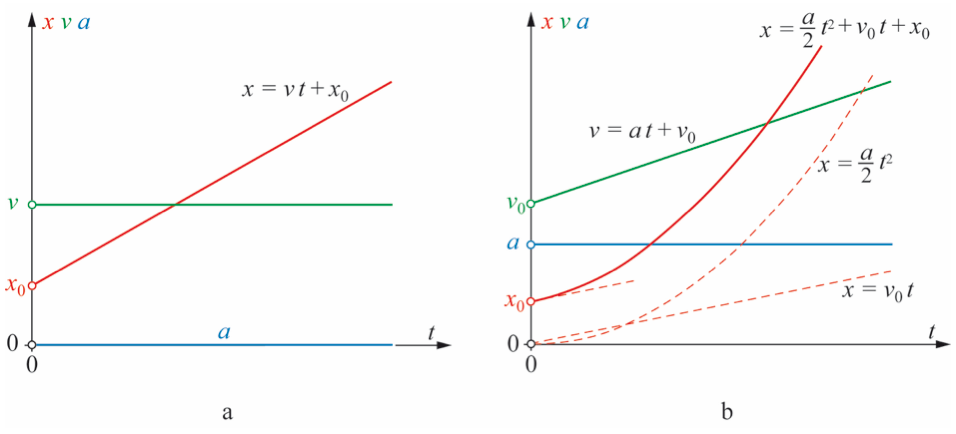
\includegraphics[width=0.7\linewidth]{images/kinematik}

\subsubsection{Translation}
\begin{tabbing}
	\begin{tabu} to \linewidth {X l l}
		\toprule
		Art & Geschwindigkeit v & Beschleunigung a \\
		\midrule
		gleichförmig & konstant & 0 \\
		gleichmässig beschleunigt & ändert sicht gleichmässig & konstant \\
		ungleichmässig beschleunigt & ändert sich ungleichmässig & ändert sich \\
	\end{tabu}
\end{tabbing}


\paragraph{Konstante Geschwindigkeit (gleichförmig)}

\begin{tabbing}
	\begin{tabu} to \linewidth {l X l X l X}
		\toprule
		Geschwindigkeit & $v = \frac{s}{t}$ &
		Strecke & $s = v \cdot t + s_0$ &
		Zeit & $t = \frac{s}{v}$ \\
		\bottomrule
	\end{tabu}
\end{tabbing}

\paragraph{Konstante Beschleunigung (gleichmässig)}

\begin{tabbing}
	\begin{tabu} to \linewidth {l X X}
		\toprule
		& Ohne Anfangsgeschwindigkeit & Mit Anfangsgeschwindigkeit \\
		\midrule
		Beschleunigung & 
		$a = \frac{\Delta v}{ \Delta t} = \dfrac{v^2}{2s} = \dfrac{2s}{t^2}$ &
		$a = \frac{v^2 - v_0^2}{2s}$ \\
		Geschwindigkeit & 
		$v = a \cdot t = \sqrt{2 a s}$ &
		$v = \sqrt{2a(s-s_0) + v_0^2} = a \cdot t + v_0 $ \\
		$\varnothing$ Geschwindigkeit & 
		$v_m = \frac{v_1 + v_2}{2} = \frac{at}{2} = \frac{s}{t}$ &
		 \\
		Strecke & 
		$s = \frac{v t}{2} = \frac{a t^2}{2} = \frac{v^2}{2a}$ &
		$s = \frac{1}{2} at^2 + v_0 t + s_0 = \frac{v^2 - v_0^2}{2a} $ \\
		Zeit & 
		$t = \frac{v}{a} = \sqrt{\frac{2s}{a}}$ & \\		
	\end{tabu}
\end{tabbing}

\begin{tabbing}
	\begin{tabu} to \linewidth {l X l}
		Variable & Bedeutung & SI-Einheit \\
		\midrule
		$v$ & Geschwindigkeit  & $\frac{m}{s}$ \\ 
		$a$ & Beschleunigung  & $\frac{m}{s^2}$ \\ 
		$t$ & Zeit  & $s$ \\ 
		$s$ & Strecke  & $m$ \\ 
		\bottomrule
	\end{tabu}
\end{tabbing}
\subsubsection{Rotation}

\begin{itemize}
	\item Eine Rotation heisst gleichförmig, wenn die Winkelgeschwindigkeit $\omega$ konstant ist. 
	\item Die Tangentialgeschwindigkeit ($\vec{v}=\omega r$) ist die Geschwindigkeit die in der Rotation gerade aus geht
\end{itemize}

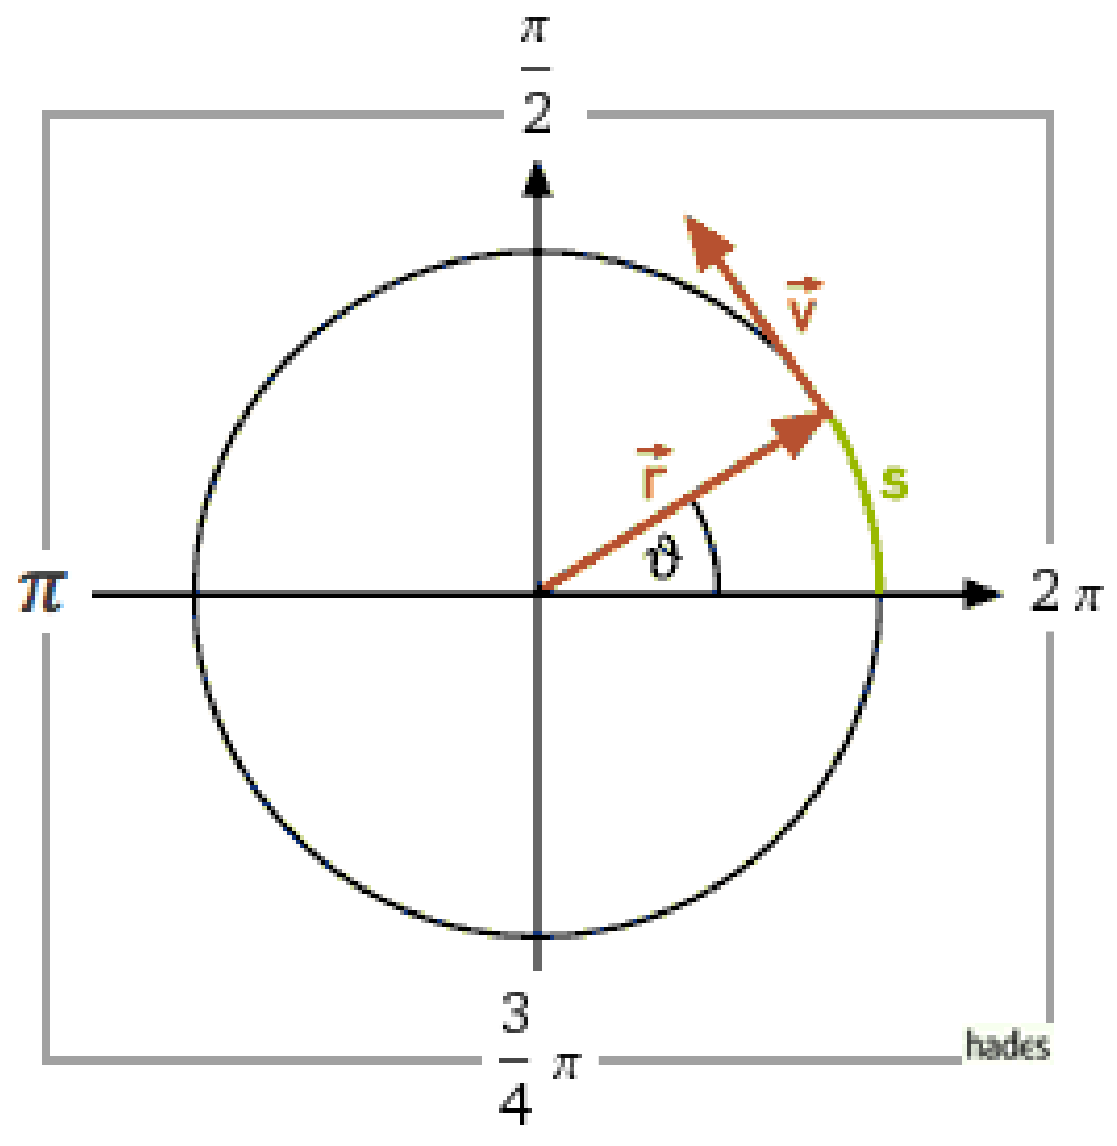
\includegraphics[width=0.2\linewidth]{images/rotation}

\paragraph{Konstante Geschwindigkeit (gleichförmig)}

\begin{tabbing}
	\begin{tabu} to \linewidth {l X l X}
		\toprule
		Winkelgeschwindigkeit & $\omega = \frac{\varphi}{t} = 2 \pi f$ &
		Rotationswinkel & $\varphi = \omega \cdot t$ \\
		Zeit & $t = \frac{\varphi}{\omega}$ &
		Drehzahl & $n = \frac{z}{t} = \frac{1}{T} = \frac{\omega}{2 \pi}$  \\
		Periodendauer & $T = \frac{1}{n} = \frac{2\pi r}{v} = \frac{2\pi}{\omega}$ &
		Anz. Umdrehungen & $N = \frac{\varphi}{2 \pi}$ \\
		\bottomrule
	\end{tabu}
\end{tabbing}

\paragraph{Konstante Beschleunigung (gleichmässig)}

\begin{tabbing}
	\begin{tabu} to \linewidth {l X X}
		\toprule
		& Ohne Anfangsgeschwindigkeit & Mit Anfangsgeschwindigkeit \\
		\midrule
		Winkelbeschleunigung & 
		$\alpha = \frac{\omega}{t} = \frac{2 \varphi}{t^2} = \frac{\omega^2}{2 \varphi}$ &
		$\alpha = \frac{\omega^2 - \omega_0^2}{2 \varphi}$ \\
		Winkelgeschwindigkeit & 
		$\omega = \alpha t = \sqrt{2 \alpha \varphi}$ &
		$\omega = \alpha t + \omega_0 = \sqrt{2\alpha \varphi + \omega_0^2} $ \\
		$\varnothing$ Winkelgeschwindigkeit & 
		$\omega_m = \frac{\alpha t}{2} = \frac{\varphi}{t}$ & \\
		Rotationswinkel & 
		$\varphi = \frac{\omega t}{2} = \frac{\omega^2}{2 \alpha} = \frac{\alpha t^2}{2} = \frac{s}{r} = 2\pi N$ &
		$\varphi = \frac{(\omega_0 + \omega_1)t}{2} = \frac{\omega^2 - \omega_0^2}{2 \alpha} = \frac{\alpha t^2}{2} + \omega_0 t + \varphi_0$ \\
	\end{tabu}
\end{tabbing}

\paragraph{Umrechnung Translation und Rotation}

\begin{tabbing}
	\begin{tabu} to \linewidth {l X l X l X}
		\toprule
		Geschwindigkeit & $v = r \cdot \omega$ &
		Beschleunigung & $a = r \cdot \alpha$ &
		Strecke & $s = r \cdot \varphi$ \\
		Winkelgeschwindigkeit & $\omega = \frac{v}{r}$ &
		Winkelbeschleunigung & $\alpha = \frac{a}{r}$ &
		Rotationswinkel & $\varphi = \frac{s}{r}$ \\
		\bottomrule
	\end{tabu}
\end{tabbing}

\begin{tabbing}
	\begin{tabu} to \linewidth {l X l}
		Variable & Bedeutung & SI-Einheit \\
		\midrule
		$\varphi$ & Rotationswinkels  & rad (Bogenmass) \\ 
		$\omega$ & Winkelgeschwindigkeit & $\frac{rad}{s}$ \\
		$\alpha$ & Winkelbeschleunigung & $\frac{rad}{s^2}$ \\
		$n = f$ & Drehzahl rsp. Umdrehungsfrequenz & $\frac{1}{s} = Hz$ \\
		$N$ & Anzahl ausgeführte Umdrehungen & \\
		$T$ & Periodendauer, Umlaufdauer & $s$ \\
		$t$ & Zeit die für die Drehung um den Winkel $\varphi$ benötigt wird & $s$ \\
		$s$ & Weg beim Umfang & $m$ \\
		$r$ & Radius & $m$ \\
		$z$ & Anzahl der Umdrehungen während der Zeit t & \\
		\bottomrule
	\end{tabu}
\end{tabbing}

\paragraph{Translation vs. Rotation}
\begin{tabbing}
	\begin{tabu} to \linewidth {l|l|l||l|l|l}
		\toprule
		& Translation & &  & Rotation &  \\ 
		\midrule
        S & Grösse & Beziehung & S & Grösse & Beziehung \\
        \midrule
        $s$ & Weg [$m$] & - & $\phi$ & Winkel [$rad$] & - \\ \hline
        $v$ & Geschwindigkeit [$\frac{m}{s}$] & $v=\frac{ds}{dt}$ & $\omega$ & Winkelgeschwindigkeit [$\frac{rad}{s}$] & $\omega = \frac{d\phi}{dt}$ \\ \hline
        $a$ & Beschleunigung [$\frac{m}{s^2}$] & $a=\frac{dv}{dt}$ & $\alpha$ & Winkelbeschleunigung [$\frac{rad}{s^2}$] & $\alpha = \frac{d\omega}{dt}$ \\ \hline
        $m$ & Masse [$kg$] & - & $J$ & Trägheitsmoment [$kg*m^2$] & - \\ \hline
        $\rho$ & Impuls [$N*s$] & $\rho = m * v$ & $L$ & Drehimpuls [$N * s$] & $L = J * \omega$ \\ \hline
        $F$ & Kraft [$N = \frac{kg*m}{s^2}$] & $F = \frac{dp}{dt}=m*a$ & $M$ & Drehmoment [$Nm$] & $M = \frac{dL}{dt} = J * \alpha$ \\ \hline
        $W$ & Arbeit [$J = N * m$] & $W = F * s$ & $W$ & Arbeit [$J = N * m$] & $W = M * \phi$ \\ \hline
        $P$ & Leistung [$W$] & $P = F*v = \frac{E}{t}$ & $P$ & Leistung [$W$] & $P = M * \omega$ \\ \hline
        $E$ & Translationsenergie [$J$] & $E_{trans} = \frac{m*v^2}{2}$ & $E$ & Rotationsenergie [$J$] & $E_{rot} = \frac{J*\omega^2}{2}$ \\ \hline
		\bottomrule
	 \end{tabu}
\end{tabbing}
\clearpage


\subsubsection{Fall und Wurf}

\paragraph{Freier Fall}
\begin{itemize}
	\item Beim freien Fall wird eine gleichmässig beschleunigte Bewegung durch die Erdanziehung hervorgerufen. ($a = g$ und $s = h$)
\end{itemize}
\begin{tabbing}
	\begin{tabu} to \linewidth {l X l X}
		\toprule
		Höhe & $h = \frac{vt}{2} = \frac{gt^2}{2}$  &
		Geschwindigkeit & $v = gt = \sqrt{2gh}$ \\
		Zeit & $t = \sqrt{\frac{2h}{g}}$ & & \\
		\bottomrule
	\end{tabu}
\end{tabbing}


\paragraph{Schiefer Wurf}

\begin{itemize}
	\item $45^\circ$ ist der optimale Winkel, falls keine Höhe überwunden werden muss!
\end{itemize}

\begin{minipage}[h!]{0.6\linewidth}
	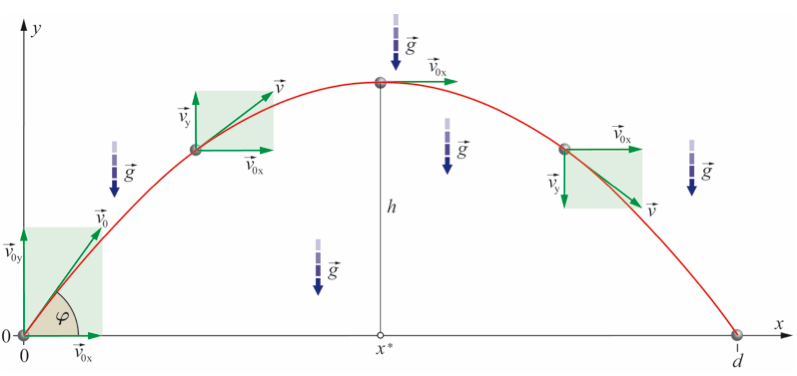
\includegraphics[width=0.9\linewidth]{images/schiefer_wurf}
\end{minipage}
\hfill
\begin{minipage}[h!]{0.4\linewidth}
Bahngleichung des Schiefen Wurfs: 
\begin{align*}
y = x \cdot tan(\varphi) - \frac{g x^2}{2 v_0^2 \cos^2(\varphi)}
\end{align*}
\end{minipage}

\begin{tabbing}
	\begin{tabu} to \linewidth {X l X l}
		\toprule
		Strecke in X & $s_x = v_0 t \cos(\alpha)$ &
		Strecke in Y & $s_y = v_0 t \sin(\alpha)  - \frac{gt^2}{2}$ \\
		Maximale Wurfhöhe & $y_{max} = \frac{v_0^2 \cdot \sin^2(\alpha)}{2g}$ &
		Maximale Wurfweite & $d = \frac{v_0^2 \cdot \sin(2\alpha)}{g}$ \\
	\end{tabu}
\end{tabbing}

\begin{tabbing}
	\begin{tabu} to \linewidth {l X}
		Momentan Geschwindigkeit & $v(t) = \sqrt{v_0^2 + g^2 t^2 - 2 v_0 \sin(\alpha) gt}$ \\
		Distanz bis zur maximale Höhe & $x_{ymax} = \frac{v_0^2 \sin^2(\alpha) \cos(\alpha)}{g} = \frac{d}{2}$ \\
		Y für bekanntes X & $y = \tan(\alpha) \cdot x - \frac{g}{2 \cdot v_0^2 \cos^2(\alpha)} \cdot x^2 $ \\
		Horizontale Geschwindigkeit & $v_x = v_0 \cdot cos(\alpha)$ \\
		Vertikale Geschwindigkeit & $v_y = v_0 \cdot sin(\alpha) - g t$ \\
	\end{tabu}
\end{tabbing}

\begin{tabbing}
	\begin{tabu} to \linewidth {l X l}
		Variable & Bedeutung & SI-Einheit \\
		\midrule
		$\alpha$ & Abwurfwinkel & $\text{Grad}^\circ$ \\ 
		$g$ & Fallbeschleunigung  & $\frac{m}{s^2}$  \\ 
		$v_0$ & Betrag der Anfangsgeschwindigkeit & $\frac{m}{s}$ \\ 
		$t$ & Zeit & $s$ \\ 
		\bottomrule
	\end{tabu}
\end{tabbing}


\vfill\null
\columnbreak

\paragraph{Senkrechter Wurf und Horizontaler Wurf} \hfill \\

\begin{itemize}
	\item Beim senkrechten Wurf gelten die Formeln des Schiefen Wurfs mit dem Winkel $\varphi = 90^\circ$
	\item Beim horizontale Wurf gelten die Formeln des Schiefen Wurfs mit dem Winkel $\varphi = 0^\circ$
\end{itemize}

\begin{minipage}[h!]{0.5\linewidth}
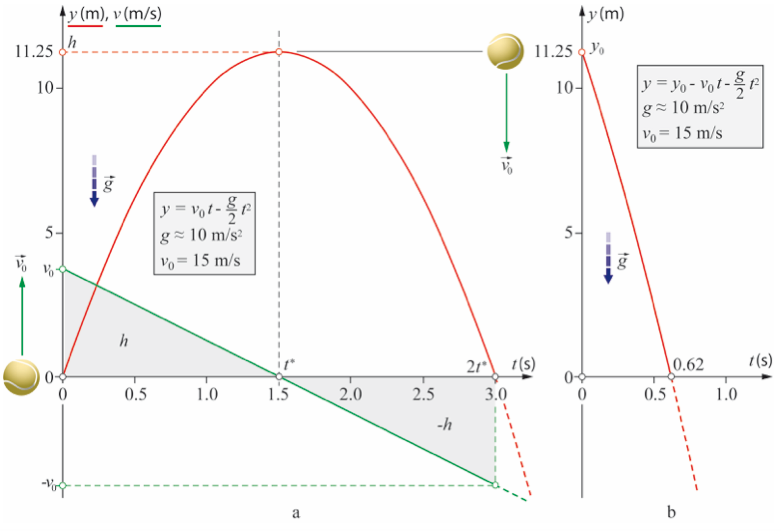
\includegraphics[width=0.9\linewidth]{images/senkrechter_wurf}
\end{minipage}
\hfill
\begin{minipage}[hbt]{0.5\linewidth}
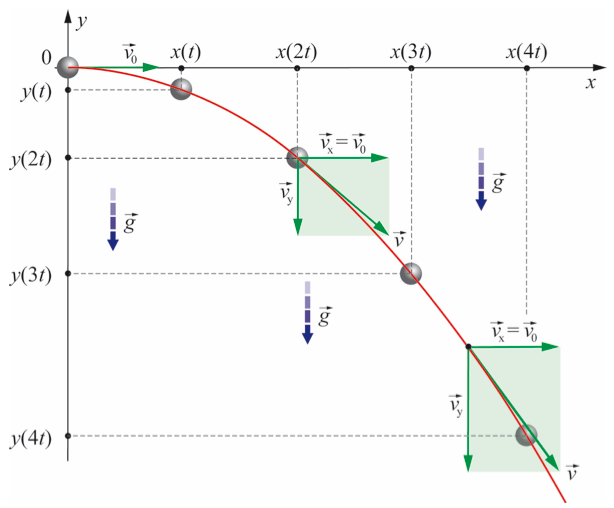
\includegraphics[width=0.9\linewidth]{images/horizontaler_wurf}
\end{minipage}



\clearpage

\subsection{Dynamik}
Die Dynamik behandelt die Kräfte als Ursache von Bewegungsabläufen. Man unterscheidet dabei die Dynamik der Translation und Rotation. (Merke: \textbf{Kraft = Gegenkraft}!)

\subsubsection{Kräfte}

\begin{itemize}
	\item Die Haft und Gleitreibung ist unabhängig von der Fläche
	\item Bei der schrägen Ebene wählt man das  Koordinaten-System mit Vorteil parallel zur Gleitebene
	\item Körper von 1kg mit $1\frac{m}{s^2}$ beschleunigen = Es wirkt eine Kraft von $1N$
	\item Beschleunigungskraft in der Schiefen Ebene: $F_B = F_H - F_G$
\end{itemize}

\begin{minipage}[h!]{0.3\linewidth}
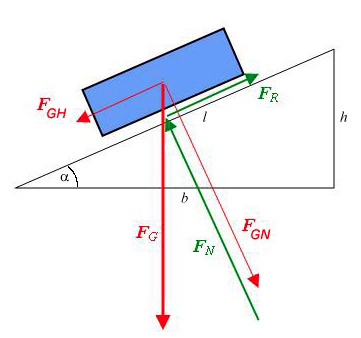
\includegraphics[width=0.9\linewidth]{images/schiefe_ebene}
\end{minipage}
\hfill
\begin{minipage}[h!]{0.2\linewidth}
	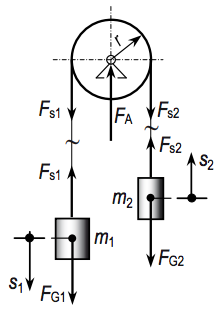
\includegraphics[width=0.9\linewidth]{images/kraefte_gleichgewicht}
\end{minipage}
\hfill
\begin{minipage}[h!]{0.4\linewidth}
\begin{align*}
m_1 \cdot a & = F_{G1} - F_{s1} \\
m_2 \cdot a & = -F_{G2} + F_{s2} \\
\Rightarrow a&=g\frac{m_1-m_2}{m_1+m_2}  \\
\Rightarrow \alpha &= \frac{a}{r} (\text{Winkelgeschwindigkeit})\\
\end{align*}
\end{minipage}

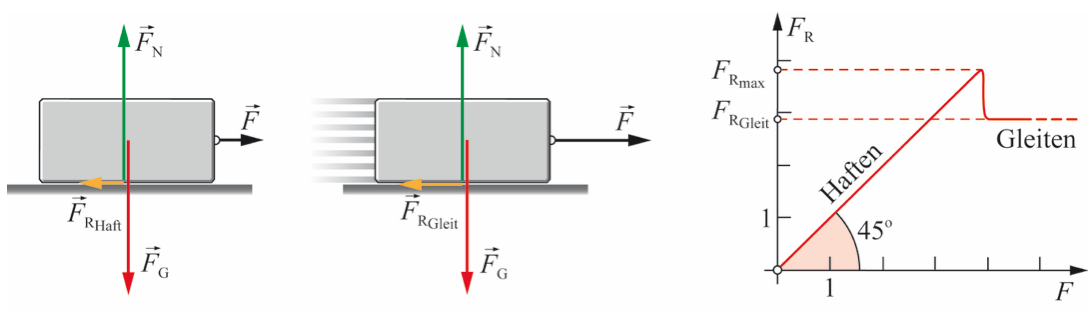
\includegraphics[width=0.9\linewidth]{images/haft_gleitkraft}


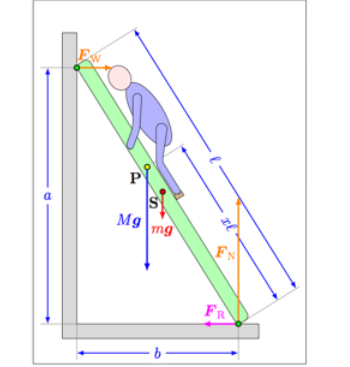
\includegraphics[width=0.3\linewidth]{images/leiter_kraefte}


\begin{tabbing}
	\begin{tabu} to \linewidth {X l X l}
		\toprule
		Kraft & $F = m \cdot a$ & 
		Kraft in Wegrichtung & $F_s = F \cos(\alpha)$ \\
		Gewichtskraft & $F_G = mg$  &
		Federkraft (Hookesches Gesetz) & $F_F = k\cdot s$ \\
		Haftreibungskraft (max) & $F_R \leq \mu_H \cdot F_N$ &
		Gleitreibungskraft & $F_R = \mu_G \cdot F_N$ \\
		Normalkraft & $F_N = mg\cdot \cos(\alpha)$ &
		Hangabtriebskraft & $F_H = F_G \cdot \sin(\alpha)$  \\
		Zentripetalkraft & $F_r = \frac{mv^2}{r} = m\omega^2r = p\omega$ & 
		Zentrifugalkraft & $F_Z = \frac{mv^2}{r} = m\omega^2r = p\omega$ \\
		Gravitationskraft & $F_G = G \cdot \frac{m_1m_2}{r^2}$
	\end{tabu}
\end{tabbing}

\begin{tabbing}
	\begin{tabu} to \linewidth {l X l}
		Variable & Bedeutung & SI-Einheit \\
		\midrule
		$F$ & Kraft & $N = \frac{kg \cdot m}{s^2}$\\ 
		$k$ & Federkonstante & $\frac{N}{m}$ \\
		$s$ & Längenänderung & $m$ \\
		$\mu_G$ & Gleitreibungskoeffizient &  \\
		$\mu_H$ & Haftreibungskoeffizient &  \\
		$G$ & Gravitationskonstante = $6.67 \cdot 10^{-11}$ & $\frac{m^3}{kg s^2}$ \\
		\bottomrule
	\end{tabu}
\end{tabbing}

\paragraph{Netwonsche Axiome}

\begin{tabbing}
	\begin{tabu} to \linewidth {l l X}
		\toprule
		I Axiom & Trägheitsprinzip & $\vec{v} = const$, wenn $ \vec{F}_{res} = \vec{0}$ \\
		II Axiom & Aktionsprinzip & $\vec{F}_{res} = m\vec{a}$\\ 
		III Axiom & Wechselwirkungsprinzip & $\vec{F}_{12} = - \vec{F}_{21}$ \\
		\bottomrule
	\end{tabu}
\end{tabbing}

\subsubsection{Arbeit}

\begin{tabbing}
	\begin{tabu} to \linewidth {l X l X}
		\toprule
		Arbeit & $W = \vec F \cdot \vec s = |\vec F| |\vec s| \cos(\alpha)\,$  &
		& \\
	\end{tabu}
\end{tabbing}

\begin{tabbing}
	\begin{tabu} to \linewidth {l X l}
		Variable & Bedeutung & SI-Einheit \\
		\midrule
		$W$ & Arbeit & $Nm = J$ \\
		$s$ & Wegstrecke & $m$ \\
		\bottomrule
	\end{tabu}
\end{tabbing}

\subsubsection{Energie}
\begin{itemize}
	\item Die Energie ist eine Zustandsgrösse eines Systems, die zunimmt, wenn von aussen Arbeit am System verrichtet wird, und die abnimmt, wenn das System nach aussen Arbeit verrichtet.
	\item Energieerhaltungssatz: Die Gesamtenergie $E_{tot}$ in einem abgeschlossenen System hat einen konstanten Wert, der von Vorgängern im Symsten nicht beeinfluss wird.
	\item Die Ausdehnung einer Feder ist proportional zur Kraft
	\item \textbf{Rollen auf der schiefen Ebene}: $E_{pot} = E_{kin} + E_{rot}$
\end{itemize}
\begin{tabbing}
	\begin{tabu} to \linewidth {l X l X}
		\toprule
		Energie & $E = P \cdot t$ & Rotationsenergie & $E_{rot} = \frac{J}{2} \cdot \omega^2 $\\
		Kinetische Energie & $E_{kin} = \frac{1}{2}mv^2$ &
		Potentielle Energie & $E_{pot} = F_G \cdot h =  mgh$ \\
		Federenergie & $E_f = \frac{F \cdot s}{2} = \frac{k \cdot s^2}{2}$ &
		Federkonstante & $k = \frac{F}{s}$ \\
	\end{tabu}
\end{tabbing}

\begin{tabbing}
	\begin{tabu} to \linewidth {l X l}
		Variable & Bedeutung & SI-Einheit \\
		\midrule
		$E$ & Energie & $J = Nm = Ws = \frac{kg \cdot m^2}{s^2}$ \\
		$k$ & Federkonstante & $\frac{N}{m}$  \\
		$s$ & Strecke welche die Feder ausgedehnt wird & $m$ \\
		$J$ & Trägheitsmoment & $J = kg \cdot m^2$ \\
		\bottomrule
	\end{tabu}
\end{tabbing}

\begin{minipage}[h!]{0.4\linewidth}
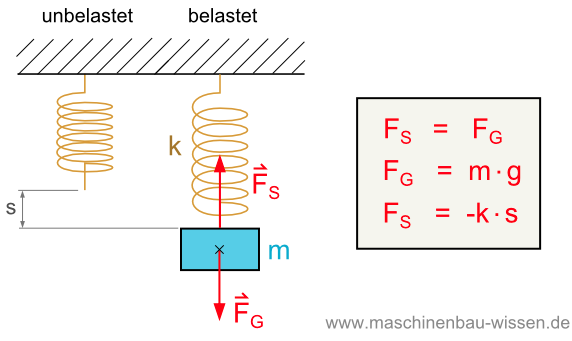
\includegraphics[width=\linewidth]{images/federenergie}
\end{minipage}
\hfill
\begin{minipage}[h!]{0.2\linewidth}
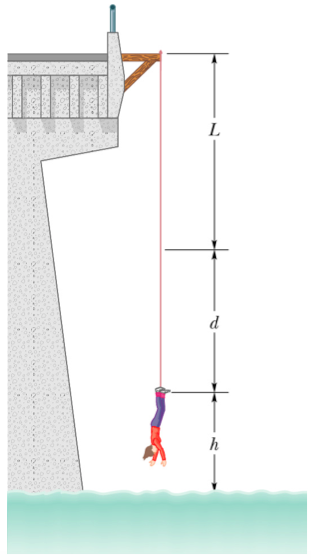
\includegraphics[width=\linewidth]{images/energie}
\end{minipage}
\hfill
\begin{minipage}[h!]{0.3\linewidth}
	\begin{align*}
	E_{pot} = E_f + E_{kin} \\
	m g (L + d) = \frac{kd^2}{2}  + \frac{m v^2}{2}  \\
	v_{Kehrpunkt} = 0 \\
	\frac{2mgL + 2mgd}{k} = d^2 \\
	d = \frac{m g}{k} \pm \frac{\sqrt{g^2 m^2 + 2 g k L m}}{k} \\
	\end{align*}
\end{minipage}

\clearpage

\subsubsection{Leistung}

\begin{tabbing}
	\begin{tabu} to \linewidth {l X l X}
		\toprule
		mittlere Leistung & $\bar{P} = \frac{W}{t}$ &
		Wirkungsgrad & $\eta = \frac{\Delta E_{ab}}{\Delta E_{zu}} = \frac{\Delta P_{ab}}{\Delta P_{zu}} < 1$ \\
		Momentanleistung & $P = F \cdot v$ & & \\
	\end{tabu}
\end{tabbing}

\begin{tabbing}
	\begin{tabu} to \linewidth {l X l}
		Variable & Bedeutung & SI-Einheit \\
		\midrule
		$P$ & Leistung & $W = \frac{J}{s} = \frac{kg \cdot m^2}{s^3}$ \\
		$E_{ab}$ & abgegebene Nutzenergie & $J$ \\
		$E_{zu}$ & aufgenommene Energie &  $J$ \\
		$W$ & verrichtete Arbeit &  $J$ \\
		$F$ & Momentankraft &  $N$ \\
		$v$ & Momentangeschwindigkeit &  $\frac{m}{s^2}$ \\
		\bottomrule
	\end{tabu}
\end{tabbing}

\paragraph{Leistung anders dargestellt}

$$P = \frac{W}{t}$$
$$W = F*s \Rightarrow P = \frac{F*s}{t}$$
$$\frac{s}{t} = v \Rightarrow P = F*v$$
$$P=\frac{\Delta E}{\Delta t}$$


\subsubsection{Impuls und Stoss}
 \textbf{Impulserhaltungssatz} In einem abgeschlossenen System bleibt der Impuls erhalten. Wenn nur Kräfte zwischen zwei Körpern wirken (Kraft = Gegenkraft) bleibt der Impuls erhalten. Die Bewegung des Schwerpunktes ändert sich nicht durch die Kollision.
 
\textbf{Elastischer Stoss}  (z.B Billiardkugel) nach dem Stoss bleibt die kinetische Energie unverändert. Der Energieerhaltungssatz für die Bewegungsenergie sowie der Impulserhaltungssatz gilt. Es geht keine Energie verloren. Der Impuls vor dem Stoss = Impuls nach dem Stoss
\begin{itemize}
	\item bewegen sich zwei Objekte aufeinander zu, ist eine Geschwindigkeit vor dem Zusammenstoss negativ.
\end{itemize}

\textbf{Unelastischer Stoss} (z.B Autounfall).
nach dem Stoss ist die kinetische Energie kleiner. (wird in Wärme und Verformungsenergie umgewandelt) (nur der Impulserhaltungssatz gilt: $p_1 + p_2 = p_1^{'} + p_2^{'}$)


\begin{tabbing}
	\begin{tabu} to \linewidth {X l X l}
		\toprule
		Impuls & $\vec{p} = m \vec{v}$  &
		Kraftstoss & $\vec{I} = \Delta \vec{p} = \vec{F} \Delta t = m \Delta \vec{v}$ \\
		Elastischer Stoss (Obj 1) & $v_1^{'} = \frac{(m_1 - m_2) \cdot v_1 + 2 m_2 v_2}{m_1+m_2}$  &
		Elastischer Stoss (Obj 2) & $v_2^{'} = \frac{(m_2 - m_1) \cdot v_2 + 2 m_1 v_1}{m_2+m_1}$ \\
		Unelastischer Stoss & $v_1^{'} = v_2^{'} = \frac{m_1v_1 + m_2v_2}{m_1 + m_2}$ & Verformungsarbeit & $W = E_1 - E_2 = \frac{m_1m_2}{2(m_1+m_2)}(v_1-v_2)^2$ \\
	\end{tabu}
\end{tabbing}

\begin{tabbing}
	\begin{tabu} to \linewidth {l X l}
		Variable & Bedeutung & SI-Einheit \\
		\midrule
		$\vec{I}$ & Kraftstoss & $Ns = \frac{kg \cdot m}{s}$ \\
		$\vec{p}$ & Impulsänderung & $Ns = \frac{kg \cdot m}{s}$ \\
		$m$ & Masse des Körpers & $kg$ \\
		$\Delta v$ & Geschwindigkeitsänderung & $\frac{m}{s}$  \\
		$F$ & beschleunigte konstante Kraft & $N$ \\
		$\Delta t$ & Dauer der Krafteinwirkung & $s$ \\
		$v^{'}$ & Geschwindigkeit des Körpers nach dem Stoss & $\frac{m}{s}$\\
		$v$ & gemeinsame Geschwindigkeit beider Körper nach dem Stoss (unelastisch) & $\frac{m}{s}$ \\
		$W$ & Verformungsarbeit & $J$\\
		$E_1$ & Summe der Bewegungsenergie beider Körper vor dem Stoss & $J$\\
		$E_2$ & Summe der Bewegungsenergie beider Körper nach dem Stoss & $J$\\
		\bottomrule
	\end{tabu}
\end{tabbing}

\paragraph{Impuls anders erklärt}

$$p = m \cdot \Delta v = m \cdot a \cdot \Delta t = F \cdot \Delta t$$

Ein Stoss überträgt Impuls, wie Arbeit Energie überträgt. Wenn man eine Kraft über eine \textit{Distanz} anwendet, macht man \textbf{Arbeit} und erhöht die \textbf{Energie}. Wenn man eine Kraft über eine \textit{Zeitdauer} anwendet, macht man einen \textbf{Stoss} und erhöht den \textbf{Impuls}.

\paragraph{Schwerpunktgeschwindigkeit}
 Die Bewegung des Schwerpunktes ändert sich nicht durch die Kollision 
 $$  u = \frac{\sum p}{ \sum m} $$

Vor dem Stoss
$$ v_{1} = u + (v_{1} -u) = u + v_{1}^{rel} $$
$$ v_{2} = u + (v_{2} -u) = u + v_{2}^{rel} $$

Elastischer Stoss
$$ v_{1} = u - (v_{1} -u) = u - v_{1}^{rel} $$
$$ v_{2} = u - (v_{2} -u) = u - v_{2}^{rel} $$
$$ E_{kin} = \frac{m_{1}+m_{2}}{2}u^2+\frac{m_{1}}{2}(v_{1}-u)^2+\frac{m_{2}}{2}(v_{2}-u)^2 $$

Inelastischer Stoss
$$ v_{1}=v_{2}=u $$
$$ E_{kin} = \frac{m_{1}+m_{2}}{2}u^2$$

\paragraph{Vollkommen inelastischer Stoss}
Die Objekte bewegen sich nachher gemeinsam weiter. Impuls ist vor und nach dem Stoss gleich

Deformationsenergie
$$ Q = E_{kin1} + E_{kin2} - (E_{kin1}^{\prime}  + E_{kin2}^{\prime})  $$

\subsubsection{Dynamik der Drehbewegung}
\begin{itemize}
	\item Zentripetalkraft (Ursache für Zentralbewegung) und Zentrifugalkraft (Fliehkraft) sind gleich gross, aber entgegengerichtet.
	\item Trägheitsmoment: Bei einem drehbaren Körper ist das Verhältnis von wirkendem Drehmoment zur erzielten Winkelbeschleunigung eine konstante Grösse, dem Trägheitsmoment.
\end{itemize}
\begin{tabbing}
	\begin{tabu} to \linewidth {X l X l}
		\toprule
		Trägheitsmoment & $J = r^2\Delta m$ &
		Trägheitsmoment & $J = \sum_{i=1}^{n}r_i^2 \Delta m_i$ \\
		Zentripetalkraft & $F_r = F_z = \frac{mv^2}{r} = m\omega^2r = p\omega$ & 
		Zentripetalbeschl & $a_r = a_z = r \omega^2 = \frac{v^2}{r}$ \\
		Rotationsleistung & $P = M \omega$ &
		Rotationenergie & $E_{rot} = \frac{J\omega^2}{2}$\\
		Drehmoment & $M = J\alpha$ &
		Rotationsarbeit & $W = M\varphi$ \\
		Drehimpuls & $L = J \omega = M \cdot t = r\cdot p$ & 
		Drehimpuls einer Punktmasse & $\Delta M = \frac{\Delta L}{\Delta t}$ \\
	\end{tabu}
\end{tabbing}

\begin{tabbing}
	\begin{tabu} to \linewidth {l X l}
		Variable & Bedeutung & SI-Einheit \\
		\midrule
		$J$ & Trägheitsmoment & $J = kg \cdot m^2$ \\ 
		$m$ & Masse eines dünnen Kreisringes (Umfang) & $kg$ \\ 
		$r$ & einheitlicher Abstand aller Massenelemente von der Drehachse & $m$ \\ 
		$m_i$ & Massenelement & $kg$\\ 
		$P$ & Leistung & $W$ \\ 
		$p$ & Impuls des Körpers & $N \cdot s$ \\
		$M$ & Drehmoment, das die Drehung verursacht & $N \cdot m$ \\ 
		$\omega$ & Winkelgeschwindigkeit des Körpers & $\frac{rad}{s} = \frac{1}{s}$ \\ 
		$L$ & Drehimpuls des rotierenden Körpers & $\frac{kg \cdot m^2}{s} = N \cdot m \cdot s$  \\ 
		$\alpha$ & Winkelbeschleunigung & $\frac{rad}{s^2} = \frac{1}{s^2}$ \\
		\bottomrule
	\end{tabu}
\end{tabbing}



\begin{minipage}[h!]{0.5\linewidth}
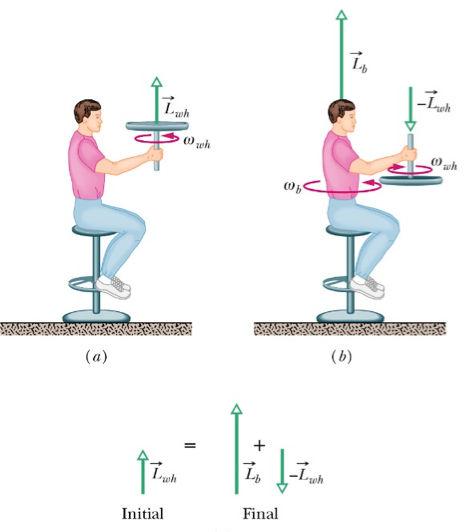
\includegraphics[width=0.8\linewidth]{images/drehimpuls}
\end{minipage}
\hfill
\begin{minipage}[h!]{0.5\linewidth}
	\begin{align*}
		L_b &= J_b \omega_b \\
		L_{wh} &= J_{wh} \omega_{wh} \\
		L_{wh} &= L_b - L_{wh} \\
		J_{wh} \omega_{wh} &= J_b \omega_b - J_{wg} \omega_{wg} \\
		\omega_b &= \frac{2J_{wh}}{J_b} \omega_{wg} \\
	\end{align*}
\end{minipage}


\clearpage

\section{Elektrizitätslehre}
\subsection{Elektrischer Stromkreis}
\begin{tabbing}
	\begin{tabu} to \linewidth {l X l X}
		\toprule
		Stromstärke & $I = \frac{\Delta Q}{\Delta t}$ & 
		Widerstand & $R = \frac{U}{I}$ \\
		Ohmsches Gesetz & $U = R \cdot I$ & 
		Widerstand eines Drahtes & R = $\frac{\rho_{el}*l}{A}$ \\
		Elektrische Leistung & $P = UI = \frac{U^2}{R} = I^2 R$ & 
		Elektrische Arbeit & $W = UI\Delta t$ \\
		Stromkosten & $K = W \cdot T$ & \\
		Kapazität Kondensators & $C= \frac{\varepsilon A}{d} \Leftrightarrow Q = CU$ &
		El. Energie Kondensator & $E=\frac{1}{2} CU^2$\\
		Geflossene Ladung & $Q = n * e$ & & \\
	\end{tabu}
\end{tabbing}


\begin{tabbing}
	\begin{tabu} to \linewidth {l X l}
		Variable & Bedeutung & SI-Einheit \\
		\midrule
		$U$ & Spannung& $V$ \\
		$R$ & Widerstand & $\Omega$ \\
		$l$ & Länge des Drahtes & \\
		$\rho_{el}$ & spezifischer Widerstand & \\
		$I$ & Stromstärke & $A$ \\
		$Q$ & geflossene Ladung & $As = C \text{ (couloumb)}$ \\
		$P$ & Leistung & $W$ \\	
		$W$ & Arbeit & $Ws / kwH$ \\
		$T$ & Tarif & $\frac{CHF}{kWh}$ \\
		$K$ & Kosten & $CHF$ \\
		\bottomrule
	\end{tabu}
\end{tabbing}

\begin{tabular}{|l|l|}
Ladung & $q = I t$
\end{tabular}

\subsection{Coulomb Gesetz}
Kraft zwischen zwei Ladungen 

$$ F=\frac{1}{4\pi\epsilon_{0}}\frac{q_{1}q_{2}}{r^2} $$

Gleiche Ladungen stossen sich ab und ungleiche ziehen sich an

\subsection{Elektrisches Feld}

$$ E =\frac{1}{4\pi\epsilon_{0}}\frac{q_{0}}{r^2}\frac{r}{r} $$ todo letzter bruch?
$$ F = qE $$

\subsection{Elektrisches Potential (Potentialunterschied)}

todo

$$ U = R*I $$

\subsection{Widerstand}


$$ R = \frac{l}{\sigma A} = \frac{\rho l}{A} [R]$$

$\sigma$ ist die Leitfähigkeit, $l$ die Länge, $A$ die Fläche des Widerstandes und $\rho$ der spezifische(material) Widerstand.\\
$$\Omega = \frac{V}{A}$$

\subsection{Elektrische Leistung (Verlustleistung)}

Wirkleistung (mechanische Leistung): Die Leistung, die letztendlich genutzt wird. \\
Scheinleistung: Die Leistung, die aus der Messung der Spannung und der Stromstärke errechnet werden kann. \\

$$ P = U*I = R * I^2 $$ 


Leistungsfaktor
$$\frac{P_{W}}{P_{S}} = cos(\phi)$$
mit $\phi$ als Phasenverschiebung

Blindleistung: $P_S*\sin\alpha$

\begin{tabular}{|ll|l|}
Scheinleistung & $S = UI$ & $[P] = VA$ \\
Wirkleistung & $P = UI \cos{\Phi}$ & $[P] = W$ \\
Blindleistung & $Q = UI \sin{\Phi}$ & $[Q] = var$
\end{tabular}



\subsection{Schaltkreise}

\subsubsection{Kirchhoffsche Gesetze}
Die Summe der Ströme in jedem Knoten ist null

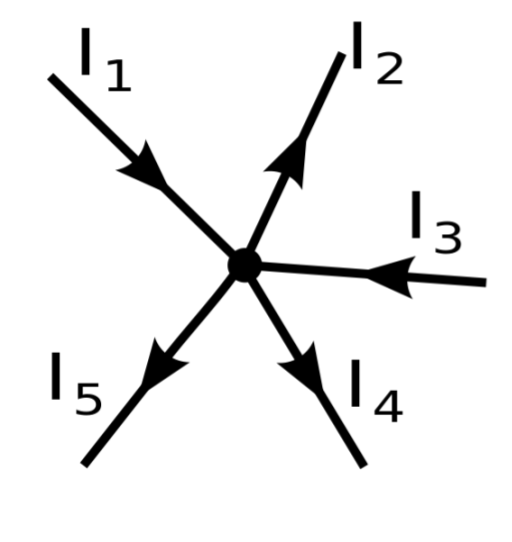
\includegraphics[scale=.3]{images/kirch1.PNG}

$$ \sum I_{k} = 0 $$

Die Summe der Teilspannungen ist null 

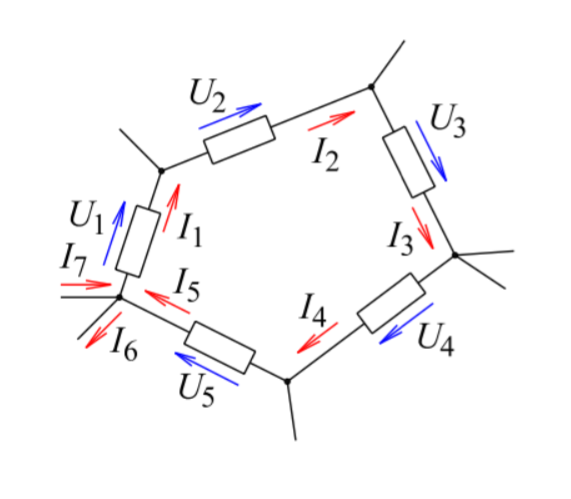
\includegraphics[scale=.3]{images/kirch2.PNG}
$$ \sum U_{k} = 0 $$

\subsubsection{Widerstände}
Reihenschaltung
$$ R_{ges} = R_1 + R_2 + R_3$$
Parallelschaltung
$$ R_{ges} = (\frac{1}{R_1}+\frac{1}{R_2}+\frac{1}{R_3})^{-1} $$



\subsection{Plattenkondensator}


\begin{tabular}{ll}
Kapazität & $  C = \frac{Q}{U} = \frac{\epsilon A}{d} $ \\
Energie & $ E = \frac{1}{2}CU^2 $ \\
Ladung & $Q = \int I(t) dt$ \\
Spannung & $U_C = \frac{\int I(t) dt}{C} = \frac{Q}{C}$
\end{tabular}


\subsection{Magnetfeld}


\begin{tabular}{|ll|l|}
Magnetische Feldstärke & $ H(r) = \frac{1}{2 \pi r} $ & $  = \frac{A}{m}$\\
Magnetische Flussdichte & $ B(r) = \frac{\mu_{0}I}{2\pi r} =  \mu_{0}H$ & $ [B] = 1T = \frac{Vs}{m^2}$ \\
Lorentzkraft (Kraft von Magnetfeld auf Ladung) & $ F = qvB $
\end{tabular}


\subsubsection{Spule}


\begin{tabular}{|ll|l|}
Magnetische Feldstärke & $H = N\frac{I}{l|}$\\
Magnetischer Fluss & $ \Phi = BA $ \\
Induktivität & $ L = N \frac{\Phi}{I} = N^2 \mu_{0} \frac{A}{l|}$ & $[L] = 1H = 1 \frac{Vs}{A}$ \\
& $ A = \pi  (\frac{Durchmesser}{2})^2$ \\
Spannung & $U = L \dot{I}$
\end{tabular}

\subsubsection{Wechselspannung und Wechselstrom}
$$U_{eff} = \frac{U_{max}}{\sqrt{2}}$$
$$I_{eff} = \frac{I_{max}}{\sqrt{2}}$$

\subsubsection{Ohmsches Gesetz der Wechselspannung}
induzierter Blindwiderstand (Spule):
$$R_{L} = \omega L$$ \\
kapazitiver Blindwiderstand (Kondensator):
$$R_{C} = \frac{-1}{\omega C}$$

\subsection{Transformator}
Bei einem Transformator mit einer Primär- und einer Sekundärwicklung, kann man das Verhältnis der Anzahl Windungen der Wicklungen in Relation zum Verhältnis der einzelnen Spannungen setzen.

$$\frac{U_{1}}{U_{2}}=\frac{N_{1}}{N_{2}}$$

dadurch kann man dann z.B. die an der zweiten Wicklung induzierte Spannung berechnen: 

$$U_{2} = U_{1} * \frac{N_{2}}{N_{1}}$$


\clearpage

\section{Differntialgleichungen}

\subsection{Analytische Lösung}
\begin{enumerate}
    \item Homogenelösung $ y^{\prime \prime}(t) + by^{\prime}(t) + cy(t) = 0 $
    \item Partikulärlösung  $ y^{\prime \prime}(t) + by^{\prime}(t) + cy(t) = f(n) $
    \item Vollständige $ y(t) = y_{p}(t) + y_{h}(t) $
\end{enumerate}

\subsubsection{Vorgehen anhand Beispiel}
\begin{enumerate}
    \item Vorgegeben Differntialgleichung $ y^{\prime} + ay(t) = b $
    \item Homogenelösung suchen  $ y^{\prime} + ay(t) = 0 $
    \begin{enumerate}
        \item Ansatz wird vorgegeben $y_{h} = Ce^{kt}$
        \item Benötigte Ableitungen von Ansatz $y_{h}$ bilden 
        \item Ableitungen in Homogenelösung einsetzten und auflösen nach Variable
        \item $y_{h}$ = Ansatz und k durch Lösung von oben ersetzt
    \end{enumerate}
    \item Partikulärlösung suchen  $ y^{\prime} + ay(t) = b $
        \begin{enumerate}
        \item Ansatz wird vorgegeben $y_{p} =\frac{b}{a}$
        \item Benötigte Ableitungen von Ansatz $y_{p}$ bilden 
        \item Ableitungen in Partikulärlösung einsetzten und auflösen
        \item $y_{p}$ = Ansatz und Variable durch Lösung von oben ersetzt
    \end{enumerate}
    \item Vollständige $ y(t) = y_{p}(t) + y_{h}(t) $
\end{enumerate}

\subsection{Nummerische Lösung}
\subsubsection{1-Ordnung}
\textbf{Euler-Verfahren}
$$ f^{\prime}(t) \approx \frac{f(t+\Delta t) - f(t)}{\Delta t} $$
$$ f^{\prime}(t) \approx \frac{f_{n+1}-f_{n}}{\Delta t}$$

\textbf{Vorgehen}
\begin{enumerate}
    \item Differentialgleichung aufstellen / vorgegeben
    \item Ableitung durch Formel oben ersetzten
    \item Auflösen nach $f_{n+1}$
\end{enumerate}

\subsubsection{2-Ordnung}
Gegeben Differentialgleichung mit 2ter Ableitung (Nach 2te Ableitung aufgelöst)
$$ y^{\prime\prime} = v^{\prime} = g-\frac{k}{m} y(t) $$

Definiere Zwischenschritt
$$ y^{\prime} = v(t) $$

Darstellen als Vektoren/Matrizen-Gleichungssystem 
$$ U^{\prime}(t) = MU(t) + b $$

Vektor definieren (1 Reihe Stammfunktion, 2 Reihe 1 Ableitung)
$$ \vec{U}(t) = \begin{bmatrix} y(t) \\ v(t) \end{bmatrix} $$
 
Matrix definieren(1 Spalte Faktoren für  Stammfunktion, 2 Spalte Faktoren für 1 Ableitung, 1 Reihe Zwischenschritt, 2 Reihe Differentialgleichung)

$$ M = \begin{bmatrix} 0 & 1 \\ -\frac{k}{m} & 0 \end{bmatrix} $$

Konstantenvektor definieren (Konstanten einsetzten: 1 Reihe Hilfsfunktion, 2 Reihe Differentialgleichungen
 $$ \vec{b} = \begin{bmatrix} 0 \\ g \end{bmatrix} $$

Nun kann nach 1-Ordnung vorgegangen werden

\clearpage

\section{Sammelsurium}

\subsection{Umrechnungen/Einheiten}
\paragraph{Einheiten}
\begin{tabbing}
	\begin{tabu} to \linewidth {l l X}
		\toprule
		Vorsatz & Vorzeichen & Faktor \\
		\midrule
		Atto  & a & $10^{-18}$ \\
		Femto & f & $10^{-15}$ \\
		Pico & p & $10^{-12}$ \\
		Nano & n & $10^{-9}$ \\
		Mikro & $\mu$ & $10^{-6}$ \\
		Milli & m & $10^{-3}$ \\
		Zenti & c & $10^{-2}$ \\
		Dezi & d & $10^{-1}$ \\
		Hekto & h & $10^{2}$ \\
		Kilo & k & $10^{3}$ \\
		Mega & M & $10^{6}$ \\
		Giga & G & $10^{9}$ \\
		Tera & T & $10^{12}$\\
		Peta & P & $10^{15}$\\
		Exa & E & $10^{18}$ \\
		\bottomrule
	 \end{tabu}
\end{tabbing}


\newpage

\paragraph{Translation vs. Rotation} (TODO an einen Ort schieben, wo man es auch findet...)



\section{Gravitation}

\begin{tabbing}
	\begin{tabu} to \linewidth {l X}
		\toprule
		Name & Formel \\
		\midrule
		Gravitationskraft  & $ F_{G}(r) = G\frac{m_{1}m_{2}}{r^2} $ \\
		Gravitationspotential & $V_{G}(r) =  -G\frac{m_{1}m_{2}}{r} $ \\
		Bedingung geschlossene Bahn (Kin + pot kleiner 0) & $ \frac{m}{2} v^2 - G\frac{mM}{r}<0$ \\
		\bottomrule
	 \end{tabu}
\end{tabbing}


\section{Sonstiges}

Dichte $$\rho = \frac{m}{V}$$
Mitternachtsformel $$\frac{-b \pm \sqrt{b^{2}-4ac}}{2a}$$

\paragraph{RPM zu $\omega$}

RPM = Rounds per Minute, RPS = Rounds per Second

$$\omega = 2\pi * rps = 2\pi * \frac{rpm}{60s}$$

Zentrifuge mit $7.5*10^4 rpm$; $\omega = \frac{7.5*10^4 rpm * 2\pi}{60s} = 7853.98 \frac{rad}{s}$

\paragraph{Joule, Nm, Ws}

$$1 J = 1 Nm = 1 \frac{W}{s}$$

\paragraph{kW zu PS}

$$1kW = 1.36PS$$

$$116 PS = 85.29kW$$

\paragraph{kcal zu Joule}

$$1 kcal = 4184 J; 1 cal = 4.184J$$

\paragraph{Looping-Formel}

$$E_{pot0} = E_{kin} + E_{pot1}$$
$$E_{pot0} = m*g*h = m*g*(h_0 + h)$$
$$E_{pot1} = m*g*h = m*g*d = m*g*2r$$
$$E_{kin} = \frac{1}{2}*m*v^2$$
$$a_z = \frac{v^2}{r} \rightarrow a_z = g \rightarrow v^2 = g*r$$
$$E_{kin} = \frac{1}{2}*m*v^2 = \frac{1}{2}*m*g*r$$
$$E_{pot0} = E_{kin} + E_{pot1}$$
$$m*g*(h_0+h) = \frac{1}{2}*m*g*r + m*g*2r$$
$$h = \frac{5}{2}r-h_0$$

Falls Höhe $h$ vorgegeben:

$$F_N = m*a$$
$$a_z = \frac{v^2}{r} = g+a = g+\frac{F_N}{m}$$
$$\frac{v^2}{r} = g+\frac{F_N}{m}$$

\subsection{Looping}
Damit der Wagen den höchsten Punkt im Looping erreicht muss die kinetische Energie $E_{\text{kin}_0}$ des Wagens vor dem Looping gleich gross sein wie die Potentielle Energie $E_{\text{pot}_0}$, die es braucht um im Looping den höchsten Punkt zu erreichen:


\begin{equation*}
\begin{aligned}
h &= \text{Höhe des Loopings (Durchmesser)} \\
E_{\text{kin}_0} &= \frac{1}{2}  m v_0^2 \\
E_{\text{pot}_0} &= mgh \\
E_{\text{kin}_0} &= E_{\text{pot}_0} 
\Leftrightarrow \frac{1}{2}  m v_0^2 = mgh 
\Leftrightarrow v_0 = \sqrt{2gh} \\
\end{aligned}
\end{equation*}

Jetzt haben wir erst berechnet wie schnell der Wagen sein muss, damit er nach oben kommt. Oben ist die Geschwindigkeit jetzt aber $0 m/s$, er fällt also wieder Runter. Darum müssen wir jetzt noch ausrechnen wie schnell der Wagen sein muss damit er nicht runterfällt. Das ist der Fall wenn die Zentrifugalkraft $F_Z$ mindestens so hoch ist wie die Erdanziehungskraft $F_G$.


\begin{equation*}
\begin{aligned}
F_Z &= \frac{mv_1^2}{r} \\
F_G &= mg \\
F_Z &= F_G 
\Leftrightarrow \frac{mv^2}{r} = mg 
\Leftrightarrow v_1 = \sqrt{g * r} = \sqrt{g * \frac{h}{2}}
\end{aligned}
\end{equation*}

Die Anfangsgeschwindigkeit muss jetzt eine genug hohe kinetische Energie $E_{\text{kin}_0}$ haben, um nach oben zu kommen $E_{\text{pot}_0}$ und genug schnell zu sein um nicht Runterzufallen $E_{\text{kin}_1}$:
\begin{equation*}
\begin{aligned}
E_{\text{kin}_0} &= E_{\text{kin}_1} + E_{\text{pot}_0} \\
\Leftrightarrow \frac{1}{2} m v_0^2 &= \frac{1}{2} m v_1^2 + mgh &| \text{ $v_1$ einsetzen} \\
\Leftrightarrow \frac{1}{2} m v_0^2 &= \frac{1}{2} m (\sqrt{g\frac{h}{2}})^2 + mgh \\
\Leftrightarrow v_0 &= \sqrt{\frac{5}{2}gh}
\end{aligned}
\end{equation*}

\paragraph{Elastische Kollisionen (Vereinfachung)}

Siehe https://www.khanacademy.org/science/physics/linear-momentum/elastic-and-inelastic-collisions/v/deriving-the-shortcut-to-solve-elastic-collision-problems und https://www.khanacademy.org/science/physics/linear-momentum/elastic-and-inelastic-collisions/v/how-to-use-the-shortcut-for-solving-elastic-collisions

\paragraph{Kopieren}

Evtl. Ableitungs-/Integralregeln aus Analysis? (abtippen)


\end{multicols*}

\end{document}
